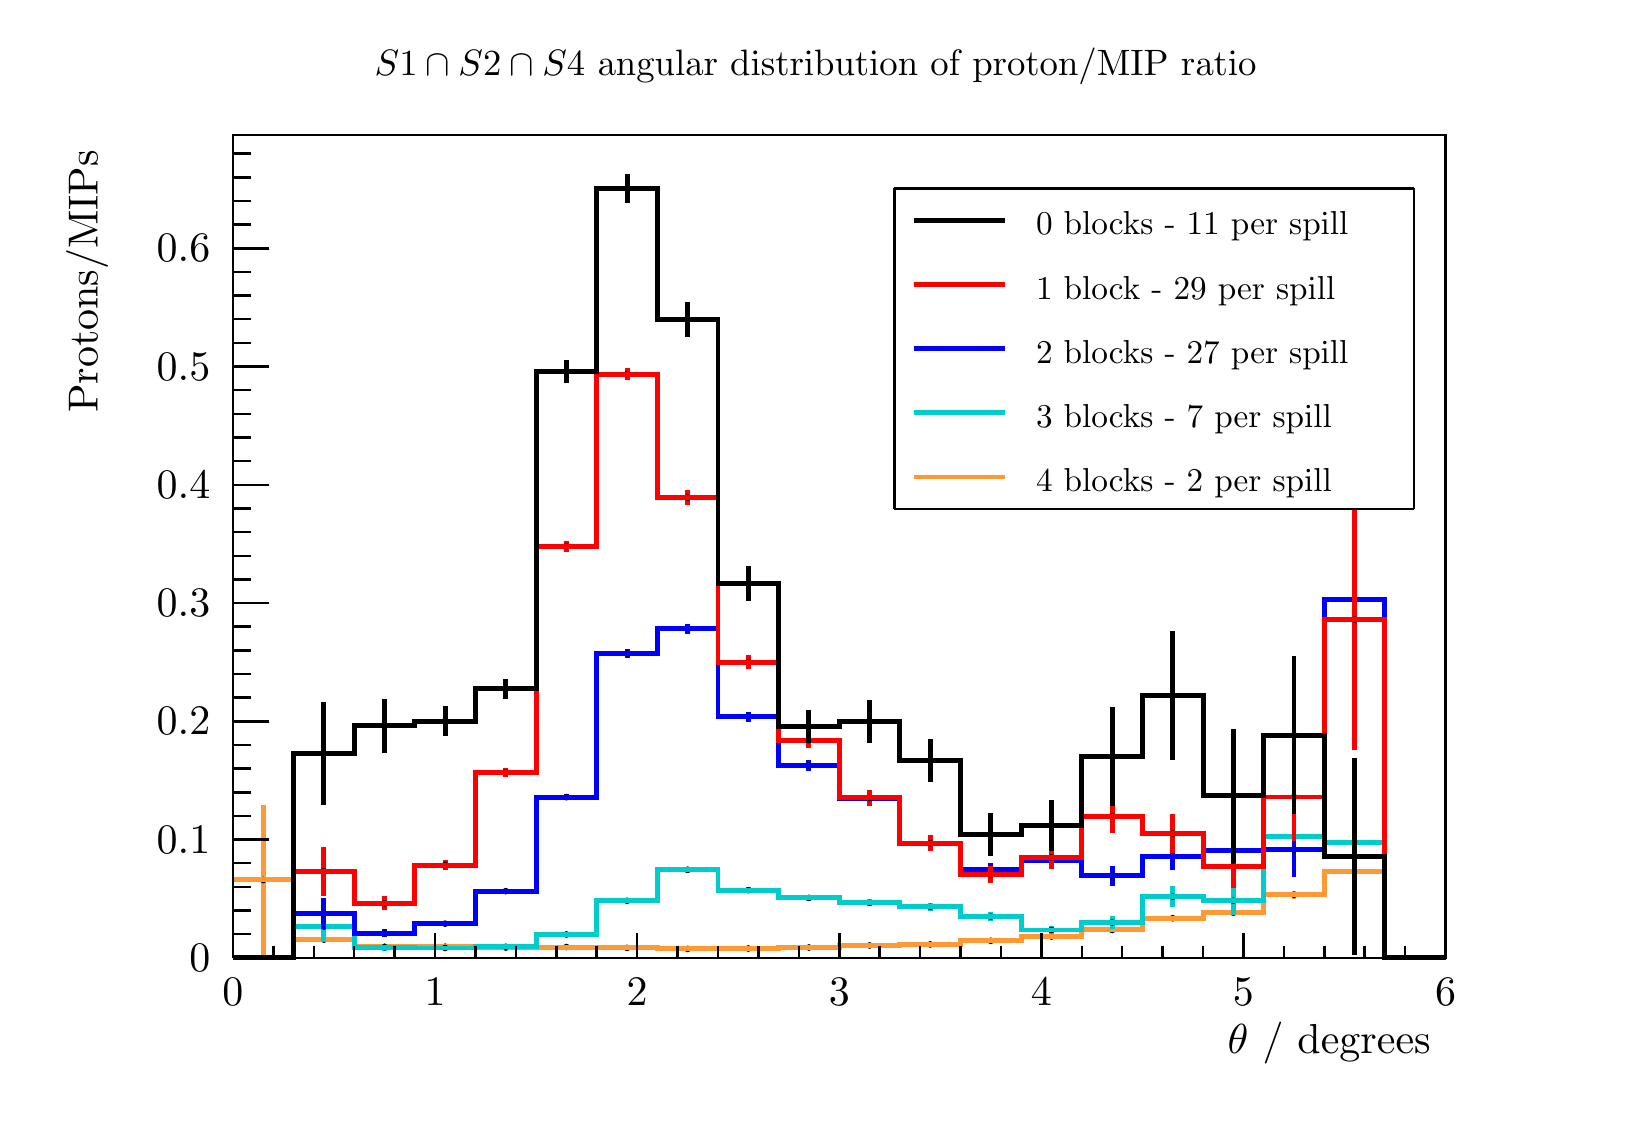
\begin{tikzpicture}
\pgfdeclareplotmark{cross} {
\pgfpathmoveto{\pgfpoint{-0.3\pgfplotmarksize}{\pgfplotmarksize}}
\pgfpathlineto{\pgfpoint{+0.3\pgfplotmarksize}{\pgfplotmarksize}}
\pgfpathlineto{\pgfpoint{+0.3\pgfplotmarksize}{0.3\pgfplotmarksize}}
\pgfpathlineto{\pgfpoint{+1\pgfplotmarksize}{0.3\pgfplotmarksize}}
\pgfpathlineto{\pgfpoint{+1\pgfplotmarksize}{-0.3\pgfplotmarksize}}
\pgfpathlineto{\pgfpoint{+0.3\pgfplotmarksize}{-0.3\pgfplotmarksize}}
\pgfpathlineto{\pgfpoint{+0.3\pgfplotmarksize}{-1.\pgfplotmarksize}}
\pgfpathlineto{\pgfpoint{-0.3\pgfplotmarksize}{-1.\pgfplotmarksize}}
\pgfpathlineto{\pgfpoint{-0.3\pgfplotmarksize}{-0.3\pgfplotmarksize}}
\pgfpathlineto{\pgfpoint{-1.\pgfplotmarksize}{-0.3\pgfplotmarksize}}
\pgfpathlineto{\pgfpoint{-1.\pgfplotmarksize}{0.3\pgfplotmarksize}}
\pgfpathlineto{\pgfpoint{-0.3\pgfplotmarksize}{0.3\pgfplotmarksize}}
\pgfpathclose
\pgfusepathqstroke
}
\pgfdeclareplotmark{cross*} {
\pgfpathmoveto{\pgfpoint{-0.3\pgfplotmarksize}{\pgfplotmarksize}}
\pgfpathlineto{\pgfpoint{+0.3\pgfplotmarksize}{\pgfplotmarksize}}
\pgfpathlineto{\pgfpoint{+0.3\pgfplotmarksize}{0.3\pgfplotmarksize}}
\pgfpathlineto{\pgfpoint{+1\pgfplotmarksize}{0.3\pgfplotmarksize}}
\pgfpathlineto{\pgfpoint{+1\pgfplotmarksize}{-0.3\pgfplotmarksize}}
\pgfpathlineto{\pgfpoint{+0.3\pgfplotmarksize}{-0.3\pgfplotmarksize}}
\pgfpathlineto{\pgfpoint{+0.3\pgfplotmarksize}{-1.\pgfplotmarksize}}
\pgfpathlineto{\pgfpoint{-0.3\pgfplotmarksize}{-1.\pgfplotmarksize}}
\pgfpathlineto{\pgfpoint{-0.3\pgfplotmarksize}{-0.3\pgfplotmarksize}}
\pgfpathlineto{\pgfpoint{-1.\pgfplotmarksize}{-0.3\pgfplotmarksize}}
\pgfpathlineto{\pgfpoint{-1.\pgfplotmarksize}{0.3\pgfplotmarksize}}
\pgfpathlineto{\pgfpoint{-0.3\pgfplotmarksize}{0.3\pgfplotmarksize}}
\pgfpathclose
\pgfusepathqfillstroke
}
\pgfdeclareplotmark{newstar} {
\pgfpathmoveto{\pgfqpoint{0pt}{\pgfplotmarksize}}
\pgfpathlineto{\pgfqpointpolar{44}{0.5\pgfplotmarksize}}
\pgfpathlineto{\pgfqpointpolar{18}{\pgfplotmarksize}}
\pgfpathlineto{\pgfqpointpolar{-20}{0.5\pgfplotmarksize}}
\pgfpathlineto{\pgfqpointpolar{-54}{\pgfplotmarksize}}
\pgfpathlineto{\pgfqpointpolar{-90}{0.5\pgfplotmarksize}}
\pgfpathlineto{\pgfqpointpolar{234}{\pgfplotmarksize}}
\pgfpathlineto{\pgfqpointpolar{198}{0.5\pgfplotmarksize}}
\pgfpathlineto{\pgfqpointpolar{162}{\pgfplotmarksize}}
\pgfpathlineto{\pgfqpointpolar{134}{0.5\pgfplotmarksize}}
\pgfpathclose
\pgfusepathqstroke
}
\pgfdeclareplotmark{newstar*} {
\pgfpathmoveto{\pgfqpoint{0pt}{\pgfplotmarksize}}
\pgfpathlineto{\pgfqpointpolar{44}{0.5\pgfplotmarksize}}
\pgfpathlineto{\pgfqpointpolar{18}{\pgfplotmarksize}}
\pgfpathlineto{\pgfqpointpolar{-20}{0.5\pgfplotmarksize}}
\pgfpathlineto{\pgfqpointpolar{-54}{\pgfplotmarksize}}
\pgfpathlineto{\pgfqpointpolar{-90}{0.5\pgfplotmarksize}}
\pgfpathlineto{\pgfqpointpolar{234}{\pgfplotmarksize}}
\pgfpathlineto{\pgfqpointpolar{198}{0.5\pgfplotmarksize}}
\pgfpathlineto{\pgfqpointpolar{162}{\pgfplotmarksize}}
\pgfpathlineto{\pgfqpointpolar{134}{0.5\pgfplotmarksize}}
\pgfpathclose
\pgfusepathqfillstroke
}
\definecolor{c}{rgb}{1,1,1};
\draw [color=c, fill=c] (0,0) rectangle (20,13.5704);
\draw [color=c, fill=c] (2.6,1.76415) rectangle (18,12.2134);
\definecolor{c}{rgb}{0,0,0};
\draw [c,line width=0.9] (2.6,1.76415) -- (2.6,12.2134) -- (18,12.2134) -- (18,1.76415) -- (2.6,1.76415);
\definecolor{c}{rgb}{1,1,1};
\draw [color=c, fill=c] (2.6,1.76415) rectangle (18,12.2134);
\definecolor{c}{rgb}{0,0,0};
\draw [c,line width=0.9] (2.6,1.76415) -- (2.6,12.2134) -- (18,12.2134) -- (18,1.76415) -- (2.6,1.76415);
\definecolor{c}{rgb}{0,0,0.6};
\draw [c,line width=0.9] (2.6,1.76415) -- (3.37,1.76415) -- (3.37,1.76415) -- (4.14,1.76415) -- (4.14,1.76415) -- (4.91,1.76415) -- (4.91,1.76415) -- (5.68,1.76415) -- (5.68,1.76415) -- (6.45,1.76415) -- (6.45,1.76415) -- (7.22,1.76415) --
 (7.22,1.76415) -- (7.99,1.76415) -- (7.99,1.76415) -- (8.76,1.76415) -- (8.76,1.76415) -- (9.53,1.76415) -- (9.53,1.76415) -- (10.3,1.76415) -- (10.3,1.76415) -- (11.07,1.76415) -- (11.07,1.76415) -- (11.84,1.76415) -- (11.84,1.76415) --
 (12.61,1.76415) -- (12.61,1.76415) -- (13.38,1.76415) -- (13.38,1.76415) -- (14.15,1.76415) -- (14.15,1.76415) -- (14.92,1.76415) -- (14.92,1.76415) -- (15.69,1.76415) -- (15.69,1.76415) -- (16.46,1.76415) -- (16.46,1.76415) -- (17.23,1.76415) --
 (17.23,1.76415) -- (18,1.76415);
\definecolor{c}{rgb}{0,0,0};
\draw [c,line width=0.9] (2.6,1.76415) -- (18,1.76415);
\draw [c,line width=0.9] (2.6,2.07763) -- (2.6,1.76415);
\draw [c,line width=0.9] (3.11333,1.92089) -- (3.11333,1.76415);
\draw [c,line width=0.9] (3.62667,1.92089) -- (3.62667,1.76415);
\draw [c,line width=0.9] (4.14,1.92089) -- (4.14,1.76415);
\draw [c,line width=0.9] (4.65333,1.92089) -- (4.65333,1.76415);
\draw [c,line width=0.9] (5.16667,2.07763) -- (5.16667,1.76415);
\draw [c,line width=0.9] (5.68,1.92089) -- (5.68,1.76415);
\draw [c,line width=0.9] (6.19333,1.92089) -- (6.19333,1.76415);
\draw [c,line width=0.9] (6.70667,1.92089) -- (6.70667,1.76415);
\draw [c,line width=0.9] (7.22,1.92089) -- (7.22,1.76415);
\draw [c,line width=0.9] (7.73333,2.07763) -- (7.73333,1.76415);
\draw [c,line width=0.9] (8.24667,1.92089) -- (8.24667,1.76415);
\draw [c,line width=0.9] (8.76,1.92089) -- (8.76,1.76415);
\draw [c,line width=0.9] (9.27333,1.92089) -- (9.27333,1.76415);
\draw [c,line width=0.9] (9.78667,1.92089) -- (9.78667,1.76415);
\draw [c,line width=0.9] (10.3,2.07763) -- (10.3,1.76415);
\draw [c,line width=0.9] (10.8133,1.92089) -- (10.8133,1.76415);
\draw [c,line width=0.9] (11.3267,1.92089) -- (11.3267,1.76415);
\draw [c,line width=0.9] (11.84,1.92089) -- (11.84,1.76415);
\draw [c,line width=0.9] (12.3533,1.92089) -- (12.3533,1.76415);
\draw [c,line width=0.9] (12.8667,2.07763) -- (12.8667,1.76415);
\draw [c,line width=0.9] (13.38,1.92089) -- (13.38,1.76415);
\draw [c,line width=0.9] (13.8933,1.92089) -- (13.8933,1.76415);
\draw [c,line width=0.9] (14.4067,1.92089) -- (14.4067,1.76415);
\draw [c,line width=0.9] (14.92,1.92089) -- (14.92,1.76415);
\draw [c,line width=0.9] (15.4333,2.07763) -- (15.4333,1.76415);
\draw [c,line width=0.9] (15.9467,1.92089) -- (15.9467,1.76415);
\draw [c,line width=0.9] (16.46,1.92089) -- (16.46,1.76415);
\draw [c,line width=0.9] (16.9733,1.92089) -- (16.9733,1.76415);
\draw [c,line width=0.9] (17.4867,1.92089) -- (17.4867,1.76415);
\draw [c,line width=0.9] (18,2.07763) -- (18,1.76415);
\draw [anchor=base] (2.6,1.15349) node[scale=1.51645, color=c, rotate=0]{0};
\draw [anchor=base] (5.16667,1.15349) node[scale=1.51645, color=c, rotate=0]{1};
\draw [anchor=base] (7.73333,1.15349) node[scale=1.51645, color=c, rotate=0]{2};
\draw [anchor=base] (10.3,1.15349) node[scale=1.51645, color=c, rotate=0]{3};
\draw [anchor=base] (12.8667,1.15349) node[scale=1.51645, color=c, rotate=0]{4};
\draw [anchor=base] (15.4333,1.15349) node[scale=1.51645, color=c, rotate=0]{5};
\draw [anchor=base] (18,1.15349) node[scale=1.51645, color=c, rotate=0]{6};
\draw [anchor= east] (18,0.678521) node[scale=1.51645, color=c, rotate=0]{$ \theta$ / degrees};
\draw [c,line width=0.9] (2.6,1.76415) -- (2.6,12.2134);
\draw [c,line width=0.9] (3.062,1.76415) -- (2.6,1.76415);
\draw [c,line width=0.9] (2.831,2.06453) -- (2.6,2.06453);
\draw [c,line width=0.9] (2.831,2.36491) -- (2.6,2.36491);
\draw [c,line width=0.9] (2.831,2.66528) -- (2.6,2.66528);
\draw [c,line width=0.9] (2.831,2.96566) -- (2.6,2.96566);
\draw [c,line width=0.9] (3.062,3.26604) -- (2.6,3.26604);
\draw [c,line width=0.9] (2.831,3.56642) -- (2.6,3.56642);
\draw [c,line width=0.9] (2.831,3.86679) -- (2.6,3.86679);
\draw [c,line width=0.9] (2.831,4.16717) -- (2.6,4.16717);
\draw [c,line width=0.9] (2.831,4.46755) -- (2.6,4.46755);
\draw [c,line width=0.9] (3.062,4.76792) -- (2.6,4.76792);
\draw [c,line width=0.9] (2.831,5.0683) -- (2.6,5.0683);
\draw [c,line width=0.9] (2.831,5.36868) -- (2.6,5.36868);
\draw [c,line width=0.9] (2.831,5.66906) -- (2.6,5.66906);
\draw [c,line width=0.9] (2.831,5.96943) -- (2.6,5.96943);
\draw [c,line width=0.9] (3.062,6.26981) -- (2.6,6.26981);
\draw [c,line width=0.9] (2.831,6.57019) -- (2.6,6.57019);
\draw [c,line width=0.9] (2.831,6.87056) -- (2.6,6.87056);
\draw [c,line width=0.9] (2.831,7.17094) -- (2.6,7.17094);
\draw [c,line width=0.9] (2.831,7.47132) -- (2.6,7.47132);
\draw [c,line width=0.9] (3.062,7.7717) -- (2.6,7.7717);
\draw [c,line width=0.9] (2.831,8.07207) -- (2.6,8.07207);
\draw [c,line width=0.9] (2.831,8.37245) -- (2.6,8.37245);
\draw [c,line width=0.9] (2.831,8.67283) -- (2.6,8.67283);
\draw [c,line width=0.9] (2.831,8.9732) -- (2.6,8.9732);
\draw [c,line width=0.9] (3.062,9.27358) -- (2.6,9.27358);
\draw [c,line width=0.9] (2.831,9.57396) -- (2.6,9.57396);
\draw [c,line width=0.9] (2.831,9.87433) -- (2.6,9.87433);
\draw [c,line width=0.9] (2.831,10.1747) -- (2.6,10.1747);
\draw [c,line width=0.9] (2.831,10.4751) -- (2.6,10.4751);
\draw [c,line width=0.9] (3.062,10.7755) -- (2.6,10.7755);
\draw [c,line width=0.9] (3.062,10.7755) -- (2.6,10.7755);
\draw [c,line width=0.9] (2.831,11.0758) -- (2.6,11.0758);
\draw [c,line width=0.9] (2.831,11.3762) -- (2.6,11.3762);
\draw [c,line width=0.9] (2.831,11.6766) -- (2.6,11.6766);
\draw [c,line width=0.9] (2.831,11.977) -- (2.6,11.977);
\draw [anchor= east] (2.5,1.76415) node[scale=1.51645, color=c, rotate=0]{0};
\draw [anchor= east] (2.5,3.26604) node[scale=1.51645, color=c, rotate=0]{0.1};
\draw [anchor= east] (2.5,4.76792) node[scale=1.51645, color=c, rotate=0]{0.2};
\draw [anchor= east] (2.5,6.26981) node[scale=1.51645, color=c, rotate=0]{0.3};
\draw [anchor= east] (2.5,7.7717) node[scale=1.51645, color=c, rotate=0]{0.4};
\draw [anchor= east] (2.5,9.27358) node[scale=1.51645, color=c, rotate=0]{0.5};
\draw [anchor= east] (2.5,10.7755) node[scale=1.51645, color=c, rotate=0]{0.6};
\draw [anchor= east] (0.746515,12.2134) node[scale=1.51645, color=c, rotate=90]{ Protons/MIPs};
\definecolor{c}{rgb}{1,0.6,0.2};
\draw [c,line width=1.8] (2.985,1.80293) -- (2.985,2.75297);
\draw [c,line width=1.8] (2.985,2.75297) -- (2.985,3.703);
\definecolor{c}{rgb}{0,0,0};
\foreach \P in {(2.985,2.75297)}{\draw[mark options={color=c,fill=c},mark size=2.402402pt,mark=*,mark size=1pt] plot coordinates {\P};}
\definecolor{c}{rgb}{1,0.6,0.2};
\draw [c,line width=1.8] (3.755,1.96233) -- (3.755,1.99599);
\draw [c,line width=1.8] (3.755,1.99599) -- (3.755,2.02966);
\definecolor{c}{rgb}{0,0,0};
\foreach \P in {(3.755,1.99599)}{\draw[mark options={color=c,fill=c},mark size=2.402402pt,mark=*,mark size=1pt] plot coordinates {\P};}
\definecolor{c}{rgb}{1,0.6,0.2};
\draw [c,line width=1.8] (4.525,1.89463) -- (4.525,1.90442);
\draw [c,line width=1.8] (4.525,1.90442) -- (4.525,1.91421);
\definecolor{c}{rgb}{0,0,0};
\foreach \P in {(4.525,1.90442)}{\draw[mark options={color=c,fill=c},mark size=2.402402pt,mark=*,mark size=1pt] plot coordinates {\P};}
\definecolor{c}{rgb}{1,0.6,0.2};
\draw [c,line width=1.8] (5.295,1.90028) -- (5.295,1.90561);
\draw [c,line width=1.8] (5.295,1.90561) -- (5.295,1.91093);
\definecolor{c}{rgb}{0,0,0};
\foreach \P in {(5.295,1.90561)}{\draw[mark options={color=c,fill=c},mark size=2.402402pt,mark=*,mark size=1pt] plot coordinates {\P};}
\definecolor{c}{rgb}{1,0.6,0.2};
\draw [c,line width=1.8] (6.065,1.89182) -- (6.065,1.89499);
\draw [c,line width=1.8] (6.065,1.89499) -- (6.065,1.89816);
\definecolor{c}{rgb}{0,0,0};
\foreach \P in {(6.065,1.89499)}{\draw[mark options={color=c,fill=c},mark size=2.402402pt,mark=*,mark size=1pt] plot coordinates {\P};}
\definecolor{c}{rgb}{1,0.6,0.2};
\draw [c,line width=1.8] (6.835,1.89866) -- (6.835,1.9013);
\draw [c,line width=1.8] (6.835,1.9013) -- (6.835,1.90395);
\definecolor{c}{rgb}{0,0,0};
\foreach \P in {(6.835,1.9013)}{\draw[mark options={color=c,fill=c},mark size=2.402402pt,mark=*,mark size=1pt] plot coordinates {\P};}
\definecolor{c}{rgb}{1,0.6,0.2};
\draw [c,line width=1.8] (7.605,1.88833) -- (7.605,1.89077);
\draw [c,line width=1.8] (7.605,1.89077) -- (7.605,1.89321);
\definecolor{c}{rgb}{0,0,0};
\foreach \P in {(7.605,1.89077)}{\draw[mark options={color=c,fill=c},mark size=2.402402pt,mark=*,mark size=1pt] plot coordinates {\P};}
\definecolor{c}{rgb}{1,0.6,0.2};
\draw [c,line width=1.8] (8.375,1.87534) -- (8.375,1.87779);
\draw [c,line width=1.8] (8.375,1.87779) -- (8.375,1.88024);
\definecolor{c}{rgb}{0,0,0};
\foreach \P in {(8.375,1.87779)}{\draw[mark options={color=c,fill=c},mark size=2.402402pt,mark=*,mark size=1pt] plot coordinates {\P};}
\definecolor{c}{rgb}{1,0.6,0.2};
\draw [c,line width=1.8] (9.145,1.8803) -- (9.145,1.88297);
\draw [c,line width=1.8] (9.145,1.88297) -- (9.145,1.88565);
\definecolor{c}{rgb}{0,0,0};
\foreach \P in {(9.145,1.88297)}{\draw[mark options={color=c,fill=c},mark size=2.402402pt,mark=*,mark size=1pt] plot coordinates {\P};}
\definecolor{c}{rgb}{1,0.6,0.2};
\draw [c,line width=1.8] (9.915,1.8927) -- (9.915,1.89581);
\draw [c,line width=1.8] (9.915,1.89581) -- (9.915,1.89892);
\definecolor{c}{rgb}{0,0,0};
\foreach \P in {(9.915,1.89581)}{\draw[mark options={color=c,fill=c},mark size=2.402402pt,mark=*,mark size=1pt] plot coordinates {\P};}
\definecolor{c}{rgb}{1,0.6,0.2};
\draw [c,line width=1.8] (10.685,1.91772) -- (10.685,1.9217);
\draw [c,line width=1.8] (10.685,1.9217) -- (10.685,1.92568);
\definecolor{c}{rgb}{0,0,0};
\foreach \P in {(10.685,1.9217)}{\draw[mark options={color=c,fill=c},mark size=2.402402pt,mark=*,mark size=1pt] plot coordinates {\P};}
\definecolor{c}{rgb}{1,0.6,0.2};
\draw [c,line width=1.8] (11.455,1.93016) -- (11.455,1.93475);
\draw [c,line width=1.8] (11.455,1.93475) -- (11.455,1.93935);
\definecolor{c}{rgb}{0,0,0};
\foreach \P in {(11.455,1.93475)}{\draw[mark options={color=c,fill=c},mark size=2.402402pt,mark=*,mark size=1pt] plot coordinates {\P};}
\definecolor{c}{rgb}{1,0.6,0.2};
\draw [c,line width=1.8] (12.225,1.97452) -- (12.225,1.98076);
\draw [c,line width=1.8] (12.225,1.98076) -- (12.225,1.98699);
\definecolor{c}{rgb}{0,0,0};
\foreach \P in {(12.225,1.98076)}{\draw[mark options={color=c,fill=c},mark size=2.402402pt,mark=*,mark size=1pt] plot coordinates {\P};}
\definecolor{c}{rgb}{1,0.6,0.2};
\draw [c,line width=1.8] (12.995,2.02664) -- (12.995,2.03532);
\draw [c,line width=1.8] (12.995,2.03532) -- (12.995,2.044);
\definecolor{c}{rgb}{0,0,0};
\foreach \P in {(12.995,2.03532)}{\draw[mark options={color=c,fill=c},mark size=2.402402pt,mark=*,mark size=1pt] plot coordinates {\P};}
\definecolor{c}{rgb}{1,0.6,0.2};
\draw [c,line width=1.8] (13.765,2.10574) -- (13.765,2.11829);
\draw [c,line width=1.8] (13.765,2.11829) -- (13.765,2.13084);
\definecolor{c}{rgb}{0,0,0};
\foreach \P in {(13.765,2.11829)}{\draw[mark options={color=c,fill=c},mark size=2.402402pt,mark=*,mark size=1pt] plot coordinates {\P};}
\definecolor{c}{rgb}{1,0.6,0.2};
\draw [c,line width=1.8] (14.535,2.24829) -- (14.535,2.26703);
\draw [c,line width=1.8] (14.535,2.26703) -- (14.535,2.28576);
\definecolor{c}{rgb}{0,0,0};
\foreach \P in {(14.535,2.26703)}{\draw[mark options={color=c,fill=c},mark size=2.402402pt,mark=*,mark size=1pt] plot coordinates {\P};}
\definecolor{c}{rgb}{1,0.6,0.2};
\draw [c,line width=1.8] (15.305,2.31094) -- (15.305,2.33717);
\draw [c,line width=1.8] (15.305,2.33717) -- (15.305,2.36339);
\definecolor{c}{rgb}{0,0,0};
\foreach \P in {(15.305,2.33717)}{\draw[mark options={color=c,fill=c},mark size=2.402402pt,mark=*,mark size=1pt] plot coordinates {\P};}
\definecolor{c}{rgb}{1,0.6,0.2};
\draw [c,line width=1.8] (16.075,2.517) -- (16.075,2.56557);
\draw [c,line width=1.8] (16.075,2.56557) -- (16.075,2.61415);
\definecolor{c}{rgb}{0,0,0};
\foreach \P in {(16.075,2.56557)}{\draw[mark options={color=c,fill=c},mark size=2.402402pt,mark=*,mark size=1pt] plot coordinates {\P};}
\definecolor{c}{rgb}{1,0.6,0.2};
\draw [c,line width=1.8] (16.845,2.75464) -- (16.845,2.86006);
\draw [c,line width=1.8] (16.845,2.86006) -- (16.845,2.96547);
\definecolor{c}{rgb}{0,0,0};
\foreach \P in {(16.845,2.86006)}{\draw[mark options={color=c,fill=c},mark size=2.402402pt,mark=*,mark size=1pt] plot coordinates {\P};}
\definecolor{c}{rgb}{1,0.6,0.2};
\draw [c,line width=1.8] (2.6,2.75297) -- (3.37,2.75297) -- (3.37,1.99599) -- (4.14,1.99599) -- (4.14,1.90442) -- (4.91,1.90442) -- (4.91,1.90561) -- (5.68,1.90561) -- (5.68,1.89499) -- (6.45,1.89499) -- (6.45,1.9013) -- (7.22,1.9013) --
 (7.22,1.89077) -- (7.99,1.89077) -- (7.99,1.87779) -- (8.76,1.87779) -- (8.76,1.88297) -- (9.53,1.88297) -- (9.53,1.89581) -- (10.3,1.89581) -- (10.3,1.9217) -- (11.07,1.9217) -- (11.07,1.93475) -- (11.84,1.93475) -- (11.84,1.98076) --
 (12.61,1.98076) -- (12.61,2.03532) -- (13.38,2.03532) -- (13.38,2.11829) -- (14.15,2.11829) -- (14.15,2.26703) -- (14.92,2.26703) -- (14.92,2.33717) -- (15.69,2.33717) -- (15.69,2.56557) -- (16.46,2.56557) -- (16.46,2.86006) -- (17.23,2.86006) --
 (17.23,1.76415) -- (18,1.76415);
\definecolor{c}{rgb}{0,0.8,0.8};
\draw [c,line width=1.8] (3.755,1.97108) -- (3.755,2.16165);
\draw [c,line width=1.8] (3.755,2.16165) -- (3.755,2.35222);
\definecolor{c}{rgb}{0,0,0};
\foreach \P in {(3.755,2.16165)}{\draw[mark options={color=c,fill=c},mark size=2.402402pt,mark=*,mark size=1pt] plot coordinates {\P};}
\definecolor{c}{rgb}{0,0.8,0.8};
\draw [c,line width=1.8] (4.525,1.85467) -- (4.525,1.89992);
\draw [c,line width=1.8] (4.525,1.89992) -- (4.525,1.94517);
\definecolor{c}{rgb}{0,0,0};
\foreach \P in {(4.525,1.89992)}{\draw[mark options={color=c,fill=c},mark size=2.402402pt,mark=*,mark size=1pt] plot coordinates {\P};}
\definecolor{c}{rgb}{0,0.8,0.8};
\draw [c,line width=1.8] (5.295,1.86685) -- (5.295,1.88929);
\draw [c,line width=1.8] (5.295,1.88929) -- (5.295,1.91173);
\definecolor{c}{rgb}{0,0,0};
\foreach \P in {(5.295,1.88929)}{\draw[mark options={color=c,fill=c},mark size=2.402402pt,mark=*,mark size=1pt] plot coordinates {\P};}
\definecolor{c}{rgb}{0,0.8,0.8};
\draw [c,line width=1.8] (6.065,1.88977) -- (6.065,1.90434);
\draw [c,line width=1.8] (6.065,1.90434) -- (6.065,1.9189);
\definecolor{c}{rgb}{0,0,0};
\foreach \P in {(6.065,1.90434)}{\draw[mark options={color=c,fill=c},mark size=2.402402pt,mark=*,mark size=1pt] plot coordinates {\P};}
\definecolor{c}{rgb}{0,0.8,0.8};
\draw [c,line width=1.8] (6.835,2.04411) -- (6.835,2.06104);
\draw [c,line width=1.8] (6.835,2.06104) -- (6.835,2.07797);
\definecolor{c}{rgb}{0,0,0};
\foreach \P in {(6.835,2.06104)}{\draw[mark options={color=c,fill=c},mark size=2.402402pt,mark=*,mark size=1pt] plot coordinates {\P};}
\definecolor{c}{rgb}{0,0.8,0.8};
\draw [c,line width=1.8] (7.605,2.46169) -- (7.605,2.4885);
\draw [c,line width=1.8] (7.605,2.4885) -- (7.605,2.51531);
\definecolor{c}{rgb}{0,0,0};
\foreach \P in {(7.605,2.4885)}{\draw[mark options={color=c,fill=c},mark size=2.402402pt,mark=*,mark size=1pt] plot coordinates {\P};}
\definecolor{c}{rgb}{0,0.8,0.8};
\draw [c,line width=1.8] (8.375,2.84625) -- (8.375,2.88349);
\draw [c,line width=1.8] (8.375,2.88349) -- (8.375,2.92072);
\definecolor{c}{rgb}{0,0,0};
\foreach \P in {(8.375,2.88349)}{\draw[mark options={color=c,fill=c},mark size=2.402402pt,mark=*,mark size=1pt] plot coordinates {\P};}
\definecolor{c}{rgb}{0,0.8,0.8};
\draw [c,line width=1.8] (9.145,2.58775) -- (9.145,2.62394);
\draw [c,line width=1.8] (9.145,2.62394) -- (9.145,2.66012);
\definecolor{c}{rgb}{0,0,0};
\foreach \P in {(9.145,2.62394)}{\draw[mark options={color=c,fill=c},mark size=2.402402pt,mark=*,mark size=1pt] plot coordinates {\P};}
\definecolor{c}{rgb}{0,0.8,0.8};
\draw [c,line width=1.8] (9.915,2.48692) -- (9.915,2.52568);
\draw [c,line width=1.8] (9.915,2.52568) -- (9.915,2.56443);
\definecolor{c}{rgb}{0,0,0};
\foreach \P in {(9.915,2.52568)}{\draw[mark options={color=c,fill=c},mark size=2.402402pt,mark=*,mark size=1pt] plot coordinates {\P};}
\definecolor{c}{rgb}{0,0.8,0.8};
\draw [c,line width=1.8] (10.685,2.41708) -- (10.685,2.46203);
\draw [c,line width=1.8] (10.685,2.46203) -- (10.685,2.50698);
\definecolor{c}{rgb}{0,0,0};
\foreach \P in {(10.685,2.46203)}{\draw[mark options={color=c,fill=c},mark size=2.402402pt,mark=*,mark size=1pt] plot coordinates {\P};}
\definecolor{c}{rgb}{0,0.8,0.8};
\draw [c,line width=1.8] (11.455,2.36192) -- (11.455,2.41133);
\draw [c,line width=1.8] (11.455,2.41133) -- (11.455,2.46074);
\definecolor{c}{rgb}{0,0,0};
\foreach \P in {(11.455,2.41133)}{\draw[mark options={color=c,fill=c},mark size=2.402402pt,mark=*,mark size=1pt] plot coordinates {\P};}
\definecolor{c}{rgb}{0,0.8,0.8};
\draw [c,line width=1.8] (12.225,2.23293) -- (12.225,2.28775);
\draw [c,line width=1.8] (12.225,2.28775) -- (12.225,2.34256);
\definecolor{c}{rgb}{0,0,0};
\foreach \P in {(12.225,2.28775)}{\draw[mark options={color=c,fill=c},mark size=2.402402pt,mark=*,mark size=1pt] plot coordinates {\P};}
\definecolor{c}{rgb}{0,0.8,0.8};
\draw [c,line width=1.8] (12.995,2.06326) -- (12.995,2.11781);
\draw [c,line width=1.8] (12.995,2.11781) -- (12.995,2.17235);
\definecolor{c}{rgb}{0,0,0};
\foreach \P in {(12.995,2.11781)}{\draw[mark options={color=c,fill=c},mark size=2.402402pt,mark=*,mark size=1pt] plot coordinates {\P};}
\definecolor{c}{rgb}{0,0.8,0.8};
\draw [c,line width=1.8] (13.765,2.13118) -- (13.765,2.21291);
\draw [c,line width=1.8] (13.765,2.21291) -- (13.765,2.29463);
\definecolor{c}{rgb}{0,0,0};
\foreach \P in {(13.765,2.21291)}{\draw[mark options={color=c,fill=c},mark size=2.402402pt,mark=*,mark size=1pt] plot coordinates {\P};}
\definecolor{c}{rgb}{0,0.8,0.8};
\draw [c,line width=1.8] (14.535,2.41042) -- (14.535,2.54139);
\draw [c,line width=1.8] (14.535,2.54139) -- (14.535,2.67235);
\definecolor{c}{rgb}{0,0,0};
\foreach \P in {(14.535,2.54139)}{\draw[mark options={color=c,fill=c},mark size=2.402402pt,mark=*,mark size=1pt] plot coordinates {\P};}
\definecolor{c}{rgb}{0,0.8,0.8};
\draw [c,line width=1.8] (15.305,2.31334) -- (15.305,2.4898);
\draw [c,line width=1.8] (15.305,2.4898) -- (15.305,2.66626);
\definecolor{c}{rgb}{0,0,0};
\foreach \P in {(15.305,2.4898)}{\draw[mark options={color=c,fill=c},mark size=2.402402pt,mark=*,mark size=1pt] plot coordinates {\P};}
\definecolor{c}{rgb}{0,0.8,0.8};
\draw [c,line width=1.8] (16.075,2.9001) -- (16.075,3.29958);
\draw [c,line width=1.8] (16.075,3.29958) -- (16.075,3.69906);
\definecolor{c}{rgb}{0,0,0};
\foreach \P in {(16.075,3.29958)}{\draw[mark options={color=c,fill=c},mark size=2.402402pt,mark=*,mark size=1pt] plot coordinates {\P};}
\definecolor{c}{rgb}{0,0.8,0.8};
\draw [c,line width=1.8] (16.845,2.40989) -- (16.845,3.23188);
\draw [c,line width=1.8] (16.845,3.23188) -- (16.845,4.05387);
\definecolor{c}{rgb}{0,0,0};
\foreach \P in {(16.845,3.23188)}{\draw[mark options={color=c,fill=c},mark size=2.402402pt,mark=*,mark size=1pt] plot coordinates {\P};}
\definecolor{c}{rgb}{0,0.8,0.8};
\draw [c,line width=1.8] (2.6,1.76415) -- (3.37,1.76415) -- (3.37,2.16165) -- (4.14,2.16165) -- (4.14,1.89992) -- (4.91,1.89992) -- (4.91,1.88929) -- (5.68,1.88929) -- (5.68,1.90434) -- (6.45,1.90434) -- (6.45,2.06104) -- (7.22,2.06104) --
 (7.22,2.4885) -- (7.99,2.4885) -- (7.99,2.88349) -- (8.76,2.88349) -- (8.76,2.62394) -- (9.53,2.62394) -- (9.53,2.52568) -- (10.3,2.52568) -- (10.3,2.46203) -- (11.07,2.46203) -- (11.07,2.41133) -- (11.84,2.41133) -- (11.84,2.28775) --
 (12.61,2.28775) -- (12.61,2.11781) -- (13.38,2.11781) -- (13.38,2.21291) -- (14.15,2.21291) -- (14.15,2.54139) -- (14.92,2.54139) -- (14.92,2.4898) -- (15.69,2.4898) -- (15.69,3.29958) -- (16.46,3.29958) -- (16.46,3.23188) -- (17.23,3.23188) --
 (17.23,1.76415) -- (18,1.76415);
\definecolor{c}{rgb}{0,0,1};
\draw [c,line width=1.8] (3.755,2.12909) -- (3.755,2.32447);
\draw [c,line width=1.8] (3.755,2.32447) -- (3.755,2.51986);
\definecolor{c}{rgb}{0,0,0};
\foreach \P in {(3.755,2.32447)}{\draw[mark options={color=c,fill=c},mark size=2.402402pt,mark=*,mark size=1pt] plot coordinates {\P};}
\definecolor{c}{rgb}{0,0,1};
\draw [c,line width=1.8] (4.525,2.02328) -- (4.525,2.07645);
\draw [c,line width=1.8] (4.525,2.07645) -- (4.525,2.12961);
\definecolor{c}{rgb}{0,0,0};
\foreach \P in {(4.525,2.07645)}{\draw[mark options={color=c,fill=c},mark size=2.402402pt,mark=*,mark size=1pt] plot coordinates {\P};}
\definecolor{c}{rgb}{0,0,1};
\draw [c,line width=1.8] (5.295,2.16334) -- (5.295,2.19826);
\draw [c,line width=1.8] (5.295,2.19826) -- (5.295,2.23317);
\definecolor{c}{rgb}{0,0,0};
\foreach \P in {(5.295,2.19826)}{\draw[mark options={color=c,fill=c},mark size=2.402402pt,mark=*,mark size=1pt] plot coordinates {\P};}
\definecolor{c}{rgb}{0,0,1};
\draw [c,line width=1.8] (6.065,2.58107) -- (6.065,2.61106);
\draw [c,line width=1.8] (6.065,2.61106) -- (6.065,2.64104);
\definecolor{c}{rgb}{0,0,0};
\foreach \P in {(6.065,2.61106)}{\draw[mark options={color=c,fill=c},mark size=2.402402pt,mark=*,mark size=1pt] plot coordinates {\P};}
\definecolor{c}{rgb}{0,0,1};
\draw [c,line width=1.8] (6.835,3.76629) -- (6.835,3.80458);
\draw [c,line width=1.8] (6.835,3.80458) -- (6.835,3.84287);
\definecolor{c}{rgb}{0,0,0};
\foreach \P in {(6.835,3.80458)}{\draw[mark options={color=c,fill=c},mark size=2.402402pt,mark=*,mark size=1pt] plot coordinates {\P};}
\definecolor{c}{rgb}{0,0,1};
\draw [c,line width=1.8] (7.605,5.57596) -- (7.605,5.62821);
\draw [c,line width=1.8] (7.605,5.62821) -- (7.605,5.68045);
\definecolor{c}{rgb}{0,0,0};
\foreach \P in {(7.605,5.62821)}{\draw[mark options={color=c,fill=c},mark size=2.402402pt,mark=*,mark size=1pt] plot coordinates {\P};}
\definecolor{c}{rgb}{0,0,1};
\draw [c,line width=1.8] (8.375,5.88159) -- (8.375,5.94342);
\draw [c,line width=1.8] (8.375,5.94342) -- (8.375,6.00526);
\definecolor{c}{rgb}{0,0,0};
\foreach \P in {(8.375,5.94342)}{\draw[mark options={color=c,fill=c},mark size=2.402402pt,mark=*,mark size=1pt] plot coordinates {\P};}
\definecolor{c}{rgb}{0,0,1};
\draw [c,line width=1.8] (9.145,4.76548) -- (9.145,4.82854);
\draw [c,line width=1.8] (9.145,4.82854) -- (9.145,4.8916);
\definecolor{c}{rgb}{0,0,0};
\foreach \P in {(9.145,4.82854)}{\draw[mark options={color=c,fill=c},mark size=2.402402pt,mark=*,mark size=1pt] plot coordinates {\P};}
\definecolor{c}{rgb}{0,0,1};
\draw [c,line width=1.8] (9.915,4.14136) -- (9.915,4.20786);
\draw [c,line width=1.8] (9.915,4.20786) -- (9.915,4.27436);
\definecolor{c}{rgb}{0,0,0};
\foreach \P in {(9.915,4.20786)}{\draw[mark options={color=c,fill=c},mark size=2.402402pt,mark=*,mark size=1pt] plot coordinates {\P};}
\definecolor{c}{rgb}{0,0,1};
\draw [c,line width=1.8] (10.685,3.71858) -- (10.685,3.79298);
\draw [c,line width=1.8] (10.685,3.79298) -- (10.685,3.86737);
\definecolor{c}{rgb}{0,0,0};
\foreach \P in {(10.685,3.79298)}{\draw[mark options={color=c,fill=c},mark size=2.402402pt,mark=*,mark size=1pt] plot coordinates {\P};}
\definecolor{c}{rgb}{0,0,1};
\draw [c,line width=1.8] (11.455,3.14004) -- (11.455,3.2137);
\draw [c,line width=1.8] (11.455,3.2137) -- (11.455,3.28736);
\definecolor{c}{rgb}{0,0,0};
\foreach \P in {(11.455,3.2137)}{\draw[mark options={color=c,fill=c},mark size=2.402402pt,mark=*,mark size=1pt] plot coordinates {\P};}
\definecolor{c}{rgb}{0,0,1};
\draw [c,line width=1.8] (12.225,2.81079) -- (12.225,2.89078);
\draw [c,line width=1.8] (12.225,2.89078) -- (12.225,2.97077);
\definecolor{c}{rgb}{0,0,0};
\foreach \P in {(12.225,2.89078)}{\draw[mark options={color=c,fill=c},mark size=2.402402pt,mark=*,mark size=1pt] plot coordinates {\P};}
\definecolor{c}{rgb}{0,0,1};
\draw [c,line width=1.8] (12.995,2.89166) -- (12.995,2.9964);
\draw [c,line width=1.8] (12.995,2.9964) -- (12.995,3.10114);
\definecolor{c}{rgb}{0,0,0};
\foreach \P in {(12.995,2.9964)}{\draw[mark options={color=c,fill=c},mark size=2.402402pt,mark=*,mark size=1pt] plot coordinates {\P};}
\definecolor{c}{rgb}{0,0,1};
\draw [c,line width=1.8] (13.765,2.6819) -- (13.765,2.80717);
\draw [c,line width=1.8] (13.765,2.80717) -- (13.765,2.93245);
\definecolor{c}{rgb}{0,0,0};
\foreach \P in {(13.765,2.80717)}{\draw[mark options={color=c,fill=c},mark size=2.402402pt,mark=*,mark size=1pt] plot coordinates {\P};}
\definecolor{c}{rgb}{0,0,1};
\draw [c,line width=1.8] (14.535,2.88376) -- (14.535,3.05518);
\draw [c,line width=1.8] (14.535,3.05518) -- (14.535,3.2266);
\definecolor{c}{rgb}{0,0,0};
\foreach \P in {(14.535,3.05518)}{\draw[mark options={color=c,fill=c},mark size=2.402402pt,mark=*,mark size=1pt] plot coordinates {\P};}
\definecolor{c}{rgb}{0,0,1};
\draw [c,line width=1.8] (15.305,2.90517) -- (15.305,3.13095);
\draw [c,line width=1.8] (15.305,3.13095) -- (15.305,3.35673);
\definecolor{c}{rgb}{0,0,0};
\foreach \P in {(15.305,3.13095)}{\draw[mark options={color=c,fill=c},mark size=2.402402pt,mark=*,mark size=1pt] plot coordinates {\P};}
\definecolor{c}{rgb}{0,0,1};
\draw [c,line width=1.8] (16.075,2.79289) -- (16.075,3.13881);
\draw [c,line width=1.8] (16.075,3.13881) -- (16.075,3.48473);
\definecolor{c}{rgb}{0,0,0};
\foreach \P in {(16.075,3.13881)}{\draw[mark options={color=c,fill=c},mark size=2.402402pt,mark=*,mark size=1pt] plot coordinates {\P};}
\definecolor{c}{rgb}{0,0,1};
\draw [c,line width=1.8] (16.845,5.25259) -- (16.845,6.31197);
\draw [c,line width=1.8] (16.845,6.31197) -- (16.845,7.37136);
\definecolor{c}{rgb}{0,0,0};
\foreach \P in {(16.845,6.31197)}{\draw[mark options={color=c,fill=c},mark size=2.402402pt,mark=*,mark size=1pt] plot coordinates {\P};}
\definecolor{c}{rgb}{0,0,1};
\draw [c,line width=1.8] (2.6,1.76415) -- (3.37,1.76415) -- (3.37,2.32447) -- (4.14,2.32447) -- (4.14,2.07645) -- (4.91,2.07645) -- (4.91,2.19826) -- (5.68,2.19826) -- (5.68,2.61106) -- (6.45,2.61106) -- (6.45,3.80458) -- (7.22,3.80458) --
 (7.22,5.62821) -- (7.99,5.62821) -- (7.99,5.94342) -- (8.76,5.94342) -- (8.76,4.82854) -- (9.53,4.82854) -- (9.53,4.20786) -- (10.3,4.20786) -- (10.3,3.79298) -- (11.07,3.79298) -- (11.07,3.2137) -- (11.84,3.2137) -- (11.84,2.89078) --
 (12.61,2.89078) -- (12.61,2.9964) -- (13.38,2.9964) -- (13.38,2.80717) -- (14.15,2.80717) -- (14.15,3.05518) -- (14.92,3.05518) -- (14.92,3.13095) -- (15.69,3.13095) -- (15.69,3.13881) -- (16.46,3.13881) -- (16.46,6.31197) -- (17.23,6.31197) --
 (17.23,1.76415) -- (18,1.76415);
\definecolor{c}{rgb}{1,0,0};
\draw [c,line width=1.8] (3.755,2.55279) -- (3.755,2.86519);
\draw [c,line width=1.8] (3.755,2.86519) -- (3.755,3.17759);
\definecolor{c}{rgb}{0,0,0};
\foreach \P in {(3.755,2.86519)}{\draw[mark options={color=c,fill=c},mark size=2.402402pt,mark=*,mark size=1pt] plot coordinates {\P};}
\definecolor{c}{rgb}{1,0,0};
\draw [c,line width=1.8] (4.525,2.36891) -- (4.525,2.45668);
\draw [c,line width=1.8] (4.525,2.45668) -- (4.525,2.54446);
\definecolor{c}{rgb}{0,0,0};
\foreach \P in {(4.525,2.45668)}{\draw[mark options={color=c,fill=c},mark size=2.402402pt,mark=*,mark size=1pt] plot coordinates {\P};}
\definecolor{c}{rgb}{1,0,0};
\draw [c,line width=1.8] (5.295,2.87772) -- (5.295,2.94232);
\draw [c,line width=1.8] (5.295,2.94232) -- (5.295,3.00693);
\definecolor{c}{rgb}{0,0,0};
\foreach \P in {(5.295,2.94232)}{\draw[mark options={color=c,fill=c},mark size=2.402402pt,mark=*,mark size=1pt] plot coordinates {\P};}
\definecolor{c}{rgb}{1,0,0};
\draw [c,line width=1.8] (6.065,4.06527) -- (6.065,4.12253);
\draw [c,line width=1.8] (6.065,4.12253) -- (6.065,4.17978);
\definecolor{c}{rgb}{0,0,0};
\foreach \P in {(6.065,4.12253)}{\draw[mark options={color=c,fill=c},mark size=2.402402pt,mark=*,mark size=1pt] plot coordinates {\P};}
\definecolor{c}{rgb}{1,0,0};
\draw [c,line width=1.8] (6.835,6.9239) -- (6.835,6.99242);
\draw [c,line width=1.8] (6.835,6.99242) -- (6.835,7.06093);
\definecolor{c}{rgb}{0,0,0};
\foreach \P in {(6.835,6.99242)}{\draw[mark options={color=c,fill=c},mark size=2.402402pt,mark=*,mark size=1pt] plot coordinates {\P};}
\definecolor{c}{rgb}{1,0,0};
\draw [c,line width=1.8] (7.605,9.09827) -- (7.605,9.17783);
\draw [c,line width=1.8] (7.605,9.17783) -- (7.605,9.25739);
\definecolor{c}{rgb}{0,0,0};
\foreach \P in {(7.605,9.17783)}{\draw[mark options={color=c,fill=c},mark size=2.402402pt,mark=*,mark size=1pt] plot coordinates {\P};}
\definecolor{c}{rgb}{1,0,0};
\draw [c,line width=1.8] (8.375,7.51961) -- (8.375,7.6101);
\draw [c,line width=1.8] (8.375,7.6101) -- (8.375,7.70058);
\definecolor{c}{rgb}{0,0,0};
\foreach \P in {(8.375,7.6101)}{\draw[mark options={color=c,fill=c},mark size=2.402402pt,mark=*,mark size=1pt] plot coordinates {\P};}
\definecolor{c}{rgb}{1,0,0};
\draw [c,line width=1.8] (9.145,5.4273) -- (9.145,5.52098);
\draw [c,line width=1.8] (9.145,5.52098) -- (9.145,5.61467);
\definecolor{c}{rgb}{0,0,0};
\foreach \P in {(9.145,5.52098)}{\draw[mark options={color=c,fill=c},mark size=2.402402pt,mark=*,mark size=1pt] plot coordinates {\P};}
\definecolor{c}{rgb}{1,0,0};
\draw [c,line width=1.8] (9.915,4.43429) -- (9.915,4.52977);
\draw [c,line width=1.8] (9.915,4.52977) -- (9.915,4.62525);
\definecolor{c}{rgb}{0,0,0};
\foreach \P in {(9.915,4.52977)}{\draw[mark options={color=c,fill=c},mark size=2.402402pt,mark=*,mark size=1pt] plot coordinates {\P};}
\definecolor{c}{rgb}{1,0,0};
\draw [c,line width=1.8] (10.685,3.69131) -- (10.685,3.79453);
\draw [c,line width=1.8] (10.685,3.79453) -- (10.685,3.89775);
\definecolor{c}{rgb}{0,0,0};
\foreach \P in {(10.685,3.79453)}{\draw[mark options={color=c,fill=c},mark size=2.402402pt,mark=*,mark size=1pt] plot coordinates {\P};}
\definecolor{c}{rgb}{1,0,0};
\draw [c,line width=1.8] (11.455,3.11979) -- (11.455,3.21926);
\draw [c,line width=1.8] (11.455,3.21926) -- (11.455,3.31873);
\definecolor{c}{rgb}{0,0,0};
\foreach \P in {(11.455,3.21926)}{\draw[mark options={color=c,fill=c},mark size=2.402402pt,mark=*,mark size=1pt] plot coordinates {\P};}
\definecolor{c}{rgb}{1,0,0};
\draw [c,line width=1.8] (12.225,2.71195) -- (12.225,2.81899);
\draw [c,line width=1.8] (12.225,2.81899) -- (12.225,2.92604);
\definecolor{c}{rgb}{0,0,0};
\foreach \P in {(12.225,2.81899)}{\draw[mark options={color=c,fill=c},mark size=2.402402pt,mark=*,mark size=1pt] plot coordinates {\P};}
\definecolor{c}{rgb}{1,0,0};
\draw [c,line width=1.8] (12.995,2.89675) -- (12.995,3.04006);
\draw [c,line width=1.8] (12.995,3.04006) -- (12.995,3.18338);
\definecolor{c}{rgb}{0,0,0};
\foreach \P in {(12.995,3.04006)}{\draw[mark options={color=c,fill=c},mark size=2.402402pt,mark=*,mark size=1pt] plot coordinates {\P};}
\definecolor{c}{rgb}{1,0,0};
\draw [c,line width=1.8] (13.765,3.34727) -- (13.765,3.56462);
\draw [c,line width=1.8] (13.765,3.56462) -- (13.765,3.78197);
\definecolor{c}{rgb}{0,0,0};
\foreach \P in {(13.765,3.56462)}{\draw[mark options={color=c,fill=c},mark size=2.402402pt,mark=*,mark size=1pt] plot coordinates {\P};}
\definecolor{c}{rgb}{1,0,0};
\draw [c,line width=1.8] (14.535,3.09242) -- (14.535,3.34445);
\draw [c,line width=1.8] (14.535,3.34445) -- (14.535,3.59648);
\definecolor{c}{rgb}{0,0,0};
\foreach \P in {(14.535,3.34445)}{\draw[mark options={color=c,fill=c},mark size=2.402402pt,mark=*,mark size=1pt] plot coordinates {\P};}
\definecolor{c}{rgb}{1,0,0};
\draw [c,line width=1.8] (15.305,2.65496) -- (15.305,2.92658);
\draw [c,line width=1.8] (15.305,2.92658) -- (15.305,3.19821);
\definecolor{c}{rgb}{0,0,0};
\foreach \P in {(15.305,2.92658)}{\draw[mark options={color=c,fill=c},mark size=2.402402pt,mark=*,mark size=1pt] plot coordinates {\P};}
\definecolor{c}{rgb}{1,0,0};
\draw [c,line width=1.8] (16.075,3.24655) -- (16.075,3.80696);
\draw [c,line width=1.8] (16.075,3.80696) -- (16.075,4.36738);
\definecolor{c}{rgb}{0,0,0};
\foreach \P in {(16.075,3.80696)}{\draw[mark options={color=c,fill=c},mark size=2.402402pt,mark=*,mark size=1pt] plot coordinates {\P};}
\definecolor{c}{rgb}{1,0,0};
\draw [c,line width=1.8] (16.845,4.4026) -- (16.845,6.05978);
\draw [c,line width=1.8] (16.845,6.05978) -- (16.845,7.71695);
\definecolor{c}{rgb}{0,0,0};
\foreach \P in {(16.845,6.05978)}{\draw[mark options={color=c,fill=c},mark size=2.402402pt,mark=*,mark size=1pt] plot coordinates {\P};}
\definecolor{c}{rgb}{1,0,0};
\draw [c,line width=1.8] (2.6,1.76415) -- (3.37,1.76415) -- (3.37,2.86519) -- (4.14,2.86519) -- (4.14,2.45668) -- (4.91,2.45668) -- (4.91,2.94232) -- (5.68,2.94232) -- (5.68,4.12253) -- (6.45,4.12253) -- (6.45,6.99242) -- (7.22,6.99242) --
 (7.22,9.17783) -- (7.99,9.17783) -- (7.99,7.6101) -- (8.76,7.6101) -- (8.76,5.52098) -- (9.53,5.52098) -- (9.53,4.52977) -- (10.3,4.52977) -- (10.3,3.79453) -- (11.07,3.79453) -- (11.07,3.21926) -- (11.84,3.21926) -- (11.84,2.81899) --
 (12.61,2.81899) -- (12.61,3.04006) -- (13.38,3.04006) -- (13.38,3.56462) -- (14.15,3.56462) -- (14.15,3.34445) -- (14.92,3.34445) -- (14.92,2.92658) -- (15.69,2.92658) -- (15.69,3.80696) -- (16.46,3.80696) -- (16.46,6.05978) -- (17.23,6.05978) --
 (17.23,1.76415) -- (18,1.76415);
\definecolor{c}{rgb}{0,0,0};
\draw [c,line width=1.8] (3.755,3.71164) -- (3.755,4.36121);
\draw [c,line width=1.8] (3.755,4.36121) -- (3.755,5.01077);
\foreach \P in {(3.755,4.36121)}{\draw[mark options={color=c,fill=c},mark size=2.402402pt,mark=*,mark size=1pt] plot coordinates {\P};}
\draw [c,line width=1.8] (4.525,4.37136) -- (4.525,4.7094);
\draw [c,line width=1.8] (4.525,4.7094) -- (4.525,5.04745);
\foreach \P in {(4.525,4.7094)}{\draw[mark options={color=c,fill=c},mark size=2.402402pt,mark=*,mark size=1pt] plot coordinates {\P};}
\draw [c,line width=1.8] (5.295,4.58419) -- (5.295,4.7717);
\draw [c,line width=1.8] (5.295,4.7717) -- (5.295,4.95922);
\foreach \P in {(5.295,4.7717)}{\draw[mark options={color=c,fill=c},mark size=2.402402pt,mark=*,mark size=1pt] plot coordinates {\P};}
\draw [c,line width=1.8] (6.065,5.05711) -- (6.065,5.18165);
\draw [c,line width=1.8] (6.065,5.18165) -- (6.065,5.30619);
\foreach \P in {(6.065,5.18165)}{\draw[mark options={color=c,fill=c},mark size=2.402402pt,mark=*,mark size=1pt] plot coordinates {\P};}
\draw [c,line width=1.8] (6.835,9.05843) -- (6.835,9.21051);
\draw [c,line width=1.8] (6.835,9.21051) -- (6.835,9.36259);
\foreach \P in {(6.835,9.21051)}{\draw[mark options={color=c,fill=c},mark size=2.402402pt,mark=*,mark size=1pt] plot coordinates {\P};}
\draw [c,line width=1.8] (7.605,11.3543) -- (7.605,11.535);
\draw [c,line width=1.8] (7.605,11.535) -- (7.605,11.7158);
\foreach \P in {(7.605,11.535)}{\draw[mark options={color=c,fill=c},mark size=2.402402pt,mark=*,mark size=1pt] plot coordinates {\P};}
\draw [c,line width=1.8] (8.375,9.65408) -- (8.375,9.87129);
\draw [c,line width=1.8] (8.375,9.87129) -- (8.375,10.0885);
\foreach \P in {(8.375,9.87129)}{\draw[mark options={color=c,fill=c},mark size=2.402402pt,mark=*,mark size=1pt] plot coordinates {\P};}
\draw [c,line width=1.8] (9.145,6.30119) -- (9.145,6.52121);
\draw [c,line width=1.8] (9.145,6.52121) -- (9.145,6.74123);
\foreach \P in {(9.145,6.52121)}{\draw[mark options={color=c,fill=c},mark size=2.402402pt,mark=*,mark size=1pt] plot coordinates {\P};}
\draw [c,line width=1.8] (9.915,4.49449) -- (9.915,4.70462);
\draw [c,line width=1.8] (9.915,4.70462) -- (9.915,4.91474);
\foreach \P in {(9.915,4.70462)}{\draw[mark options={color=c,fill=c},mark size=2.402402pt,mark=*,mark size=1pt] plot coordinates {\P};}
\draw [c,line width=1.8] (10.685,4.49315) -- (10.685,4.76884);
\draw [c,line width=1.8] (10.685,4.76884) -- (10.685,5.04452);
\foreach \P in {(10.685,4.76884)}{\draw[mark options={color=c,fill=c},mark size=2.402402pt,mark=*,mark size=1pt] plot coordinates {\P};}
\draw [c,line width=1.8] (11.455,3.99902) -- (11.455,4.27366);
\draw [c,line width=1.8] (11.455,4.27366) -- (11.455,4.54831);
\foreach \P in {(11.455,4.27366)}{\draw[mark options={color=c,fill=c},mark size=2.402402pt,mark=*,mark size=1pt] plot coordinates {\P};}
\draw [c,line width=1.8] (12.225,3.05853) -- (12.225,3.32882);
\draw [c,line width=1.8] (12.225,3.32882) -- (12.225,3.5991);
\foreach \P in {(12.225,3.32882)}{\draw[mark options={color=c,fill=c},mark size=2.402402pt,mark=*,mark size=1pt] plot coordinates {\P};}
\draw [c,line width=1.8] (12.995,3.12222) -- (12.995,3.44397);
\draw [c,line width=1.8] (12.995,3.44397) -- (12.995,3.76573);
\foreach \P in {(12.995,3.44397)}{\draw[mark options={color=c,fill=c},mark size=2.402402pt,mark=*,mark size=1pt] plot coordinates {\P};}
\draw [c,line width=1.8] (13.765,3.69441) -- (13.765,4.32181);
\draw [c,line width=1.8] (13.765,4.32181) -- (13.765,4.94921);
\foreach \P in {(13.765,4.32181)}{\draw[mark options={color=c,fill=c},mark size=2.402402pt,mark=*,mark size=1pt] plot coordinates {\P};}
\draw [c,line width=1.8] (14.535,4.27806) -- (14.535,5.09377);
\draw [c,line width=1.8] (14.535,5.09377) -- (14.535,5.90948);
\foreach \P in {(14.535,5.09377)}{\draw[mark options={color=c,fill=c},mark size=2.402402pt,mark=*,mark size=1pt] plot coordinates {\P};}
\draw [c,line width=1.8] (15.305,2.97174) -- (15.305,3.82111);
\draw [c,line width=1.8] (15.305,3.82111) -- (15.305,4.67048);
\foreach \P in {(15.305,3.82111)}{\draw[mark options={color=c,fill=c},mark size=2.402402pt,mark=*,mark size=1pt] plot coordinates {\P};}
\draw [c,line width=1.8] (16.075,3.58767) -- (16.075,4.59256);
\draw [c,line width=1.8] (16.075,4.59256) -- (16.075,5.59744);
\foreach \P in {(16.075,4.59256)}{\draw[mark options={color=c,fill=c},mark size=2.402402pt,mark=*,mark size=1pt] plot coordinates {\P};}
\draw [c,line width=1.8] (16.845,1.7978) -- (16.845,3.04932);
\draw [c,line width=1.8] (16.845,3.04932) -- (16.845,4.30084);
\foreach \P in {(16.845,3.04932)}{\draw[mark options={color=c,fill=c},mark size=2.402402pt,mark=*,mark size=1pt] plot coordinates {\P};}
\draw [c,line width=1.8] (2.6,1.76415) -- (3.37,1.76415) -- (3.37,4.36121) -- (4.14,4.36121) -- (4.14,4.7094) -- (4.91,4.7094) -- (4.91,4.7717) -- (5.68,4.7717) -- (5.68,5.18165) -- (6.45,5.18165) -- (6.45,9.21051) -- (7.22,9.21051) -- (7.22,11.535)
 -- (7.99,11.535) -- (7.99,9.87129) -- (8.76,9.87129) -- (8.76,6.52121) -- (9.53,6.52121) -- (9.53,4.70462) -- (10.3,4.70462) -- (10.3,4.76884) -- (11.07,4.76884) -- (11.07,4.27366) -- (11.84,4.27366) -- (11.84,3.32882) -- (12.61,3.32882) --
 (12.61,3.44397) -- (13.38,3.44397) -- (13.38,4.32181) -- (14.15,4.32181) -- (14.15,5.09377) -- (14.92,5.09377) -- (14.92,3.82111) -- (15.69,3.82111) -- (15.69,4.59256) -- (16.46,4.59256) -- (16.46,3.04932) -- (17.23,3.04932) -- (17.23,1.76415) --
 (18,1.76415);
\draw [c,line width=0.9] (2.6,1.76415) -- (18,1.76415);
\draw [c,line width=0.9] (2.6,2.07763) -- (2.6,1.76415);
\draw [c,line width=0.9] (3.11333,1.92089) -- (3.11333,1.76415);
\draw [c,line width=0.9] (3.62667,1.92089) -- (3.62667,1.76415);
\draw [c,line width=0.9] (4.14,1.92089) -- (4.14,1.76415);
\draw [c,line width=0.9] (4.65333,1.92089) -- (4.65333,1.76415);
\draw [c,line width=0.9] (5.16667,2.07763) -- (5.16667,1.76415);
\draw [c,line width=0.9] (5.68,1.92089) -- (5.68,1.76415);
\draw [c,line width=0.9] (6.19333,1.92089) -- (6.19333,1.76415);
\draw [c,line width=0.9] (6.70667,1.92089) -- (6.70667,1.76415);
\draw [c,line width=0.9] (7.22,1.92089) -- (7.22,1.76415);
\draw [c,line width=0.9] (7.73333,2.07763) -- (7.73333,1.76415);
\draw [c,line width=0.9] (8.24667,1.92089) -- (8.24667,1.76415);
\draw [c,line width=0.9] (8.76,1.92089) -- (8.76,1.76415);
\draw [c,line width=0.9] (9.27333,1.92089) -- (9.27333,1.76415);
\draw [c,line width=0.9] (9.78667,1.92089) -- (9.78667,1.76415);
\draw [c,line width=0.9] (10.3,2.07763) -- (10.3,1.76415);
\draw [c,line width=0.9] (10.8133,1.92089) -- (10.8133,1.76415);
\draw [c,line width=0.9] (11.3267,1.92089) -- (11.3267,1.76415);
\draw [c,line width=0.9] (11.84,1.92089) -- (11.84,1.76415);
\draw [c,line width=0.9] (12.3533,1.92089) -- (12.3533,1.76415);
\draw [c,line width=0.9] (12.8667,2.07763) -- (12.8667,1.76415);
\draw [c,line width=0.9] (13.38,1.92089) -- (13.38,1.76415);
\draw [c,line width=0.9] (13.8933,1.92089) -- (13.8933,1.76415);
\draw [c,line width=0.9] (14.4067,1.92089) -- (14.4067,1.76415);
\draw [c,line width=0.9] (14.92,1.92089) -- (14.92,1.76415);
\draw [c,line width=0.9] (15.4333,2.07763) -- (15.4333,1.76415);
\draw [c,line width=0.9] (15.9467,1.92089) -- (15.9467,1.76415);
\draw [c,line width=0.9] (16.46,1.92089) -- (16.46,1.76415);
\draw [c,line width=0.9] (16.9733,1.92089) -- (16.9733,1.76415);
\draw [c,line width=0.9] (17.4867,1.92089) -- (17.4867,1.76415);
\draw [c,line width=0.9] (18,2.07763) -- (18,1.76415);
\draw [c,line width=0.9] (2.6,1.76415) -- (2.6,12.2134);
\draw [c,line width=0.9] (3.062,1.76415) -- (2.6,1.76415);
\draw [c,line width=0.9] (2.831,2.06453) -- (2.6,2.06453);
\draw [c,line width=0.9] (2.831,2.36491) -- (2.6,2.36491);
\draw [c,line width=0.9] (2.831,2.66528) -- (2.6,2.66528);
\draw [c,line width=0.9] (2.831,2.96566) -- (2.6,2.96566);
\draw [c,line width=0.9] (3.062,3.26604) -- (2.6,3.26604);
\draw [c,line width=0.9] (2.831,3.56642) -- (2.6,3.56642);
\draw [c,line width=0.9] (2.831,3.86679) -- (2.6,3.86679);
\draw [c,line width=0.9] (2.831,4.16717) -- (2.6,4.16717);
\draw [c,line width=0.9] (2.831,4.46755) -- (2.6,4.46755);
\draw [c,line width=0.9] (3.062,4.76792) -- (2.6,4.76792);
\draw [c,line width=0.9] (2.831,5.0683) -- (2.6,5.0683);
\draw [c,line width=0.9] (2.831,5.36868) -- (2.6,5.36868);
\draw [c,line width=0.9] (2.831,5.66906) -- (2.6,5.66906);
\draw [c,line width=0.9] (2.831,5.96943) -- (2.6,5.96943);
\draw [c,line width=0.9] (3.062,6.26981) -- (2.6,6.26981);
\draw [c,line width=0.9] (2.831,6.57019) -- (2.6,6.57019);
\draw [c,line width=0.9] (2.831,6.87056) -- (2.6,6.87056);
\draw [c,line width=0.9] (2.831,7.17094) -- (2.6,7.17094);
\draw [c,line width=0.9] (2.831,7.47132) -- (2.6,7.47132);
\draw [c,line width=0.9] (3.062,7.7717) -- (2.6,7.7717);
\draw [c,line width=0.9] (2.831,8.07207) -- (2.6,8.07207);
\draw [c,line width=0.9] (2.831,8.37245) -- (2.6,8.37245);
\draw [c,line width=0.9] (2.831,8.67283) -- (2.6,8.67283);
\draw [c,line width=0.9] (2.831,8.9732) -- (2.6,8.9732);
\draw [c,line width=0.9] (3.062,9.27358) -- (2.6,9.27358);
\draw [c,line width=0.9] (2.831,9.57396) -- (2.6,9.57396);
\draw [c,line width=0.9] (2.831,9.87433) -- (2.6,9.87433);
\draw [c,line width=0.9] (2.831,10.1747) -- (2.6,10.1747);
\draw [c,line width=0.9] (2.831,10.4751) -- (2.6,10.4751);
\draw [c,line width=0.9] (3.062,10.7755) -- (2.6,10.7755);
\draw [c,line width=0.9] (3.062,10.7755) -- (2.6,10.7755);
\draw [c,line width=0.9] (2.831,11.0758) -- (2.6,11.0758);
\draw [c,line width=0.9] (2.831,11.3762) -- (2.6,11.3762);
\draw [c,line width=0.9] (2.831,11.6766) -- (2.6,11.6766);
\draw [c,line width=0.9] (2.831,11.977) -- (2.6,11.977);
\draw (10,13.0877) node[scale=1.3269, color=c, rotate=0]{$S1 \cap S2 \cap S4$ angular distribution of proton/MIP ratio};
\definecolor{c}{rgb}{1,1,1};
\draw [color=c, fill=c] (11,7.46373) rectangle (17.6,11.5349);
\definecolor{c}{rgb}{0,0,0};
\draw [c,line width=0.9] (11,7.46373) -- (17.6,7.46373);
\draw [c,line width=0.9] (17.6,7.46373) -- (17.6,11.5349);
\draw [c,line width=0.9] (17.6,11.5349) -- (11,11.5349);
\draw [c,line width=0.9] (11,11.5349) -- (11,7.46373);
\draw [anchor=base west] (12.65,10.9445) node[scale=1.20052, color=c, rotate=0]{0 blocks - 11 per spill};
\draw [c,line width=1.8] (11.2475,11.1277) -- (12.4025,11.1277);
\draw [anchor=base west] (12.65,10.1303) node[scale=1.20052, color=c, rotate=0]{1 block - 29 per spill};
\definecolor{c}{rgb}{1,0,0};
\draw [c,line width=1.8] (11.2475,10.3135) -- (12.4025,10.3135);
\definecolor{c}{rgb}{0,0,0};
\draw [anchor=base west] (12.65,9.31609) node[scale=1.20052, color=c, rotate=0]{2 blocks - 27 per spill};
\definecolor{c}{rgb}{0,0,1};
\draw [c,line width=1.8] (11.2475,9.49929) -- (12.4025,9.49929);
\definecolor{c}{rgb}{0,0,0};
\draw [anchor=base west] (12.65,8.50186) node[scale=1.20052, color=c, rotate=0]{3 blocks - 7 per spill};
\definecolor{c}{rgb}{0,0.8,0.8};
\draw [c,line width=1.8] (11.2475,8.68506) -- (12.4025,8.68506);
\definecolor{c}{rgb}{0,0,0};
\draw [anchor=base west] (12.65,7.68764) node[scale=1.20052, color=c, rotate=0]{4 blocks - 2 per spill};
\definecolor{c}{rgb}{1,0.6,0.2};
\draw [c,line width=1.8] (11.2475,7.87084) -- (12.4025,7.87084);
\end{tikzpicture}
